\documentclass[12pt,a4paper]{article}
\usepackage{geometry}
\usepackage{hyperref}
\usepackage{listings}
\lstset{language=VHDL} 
\usepackage{multirow}
\geometry{
	a4paper,
	total={170mm,257mm},
	left=20mm,
	right=20mm,
	top=20mm,
	bottom=20mm
}
\setlength{\parindent}{4em}
\setlength{\parskip}{1em}
\renewcommand{\baselinestretch}{1.3}

\usepackage{graphicx}

\usepackage{float}

\usepackage{polski}
\usepackage[utf8]{inputenc}

\usepackage{xcolor}
\colorlet{keyword}{blue!100!black!80}
\colorlet{comment}{green!90!black!90}
\lstdefinestyle{vhdl}{
   language     = VHDL,
   basicstyle   = \ttfamily,
   keywordstyle = \color{keyword}\bfseries,
   commentstyle = \color{comment}
}

\begin{document}
\begin{titlepage}
		\newgeometry{top=5cm, bottom=3cm}
		
		\centering
		{\huge\bfseries Układy Cyfrowe i Systemy Wbudowane 2\par}
		
		\vspace{0.8cm}
		{\large Prowadzący: Dr inż. Dariusz Banasiak, wtorek 11:15 TP } 
		\vfill	
		{\Large\bfseries Gra Pong \par}
		\vfill
		
		{\large\bfseries Michał Madarasz 238903\par}
		{\large\bfseries Piotr Borowski 234996\par}
		
		\vspace{1cm}
		{04 czerwiec 2019}
		
		\restoregeometry
	\end{titlepage}

	\newgeometry{top=1.5cm, bottom=1.5cm, 				left=20mm, right=20mm}
	
	
	\tableofcontents	
	
	\setlength{\parindent}{8ex}	
	
	\newpage
	

    \section{Wprowadzenie}
    \subsection{Cel i zakres}
    Celem projektu jest zaprojektowanie oraz zaimplementowanie przy użyciu języka VHDL prostej gry działającej na układzie Spartan-3E (XC3S500E). Sterowanie w grze będzie odbywać się za pomocą enkodera, a wyświetlanie obrazu gry przy użyciu monitora VGA. 
    
Projekt zostanie przeprowadzony w sposób iteracyjny, z podziałem na etapy mające na celu stopniowe poznawanie potrzebnych technologii i ich zastosowanie w projekcie. Można wyróżnić następujące etapy: 
\begin{enumerate}
    \item Nawiązanie komunikacji z monitorem VGA
    \item Nawiązanie komunikacji z enkoderem
    \item Określenie oraz implementacja mechaniki gry
\end{enumerate}
Każdemu etapowi będą towarzyszyły testy, mające na celu sprawdzenie, czy kolejne funkcjonalności zostały zrealizowane poprawnie oraz testy weryfikujące grywalność gry.

\subsection{Mechanika gry}
Podczas projektu postaramy się utworzyć grę zręcznościową, w której gracz będzie przy pomocy enkodera poruszał paletką.
\subsubsection{Cel gry}
Gracz będzie miał na celu odbijanie wygenerowanej piłeczki tak, by nie znalazła się ona poniżej położenia paletki. Piłeczka będzie odbijała się od krawędzi ekranu. Po przegranej gra zaczyna się od początku.
\subsubsection{Statystyki}
Gra będzie wyświetlała na ekranie statystyki gry: liczbę odbić, liczbę przegranych.

\subsection{Sprzęt}
Projekt został zaimplementowany na płycie Spartan-3E (UG230). Z punktu widzenia projektu istotnymi układami umieszczonymi na tej płycie były: układ FPGA XC3S500E, zegar 50MHz, port VGA oraz RotaryEncoder.

\subsection{Schemat logiczny}
\begin{center}
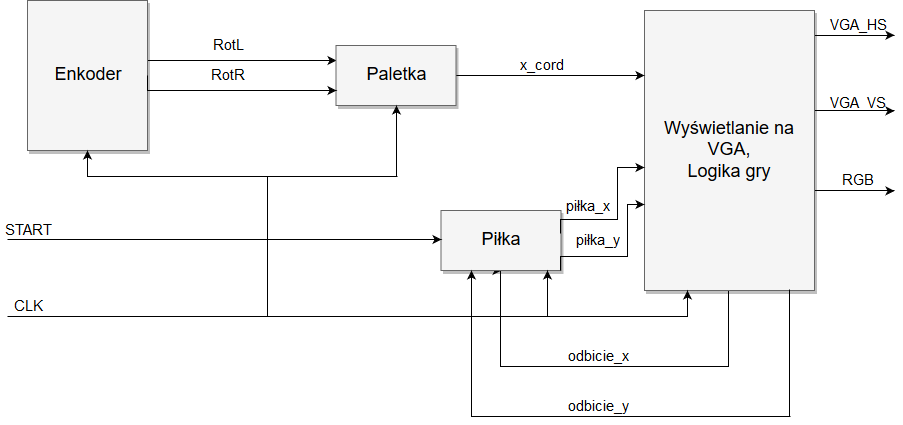
\includegraphics[width=16cm, height=8cm]{schametzalozenia.png}    
\end{center}

Sygnały:
\begin{itemize}
\item START (std\_logic) – sygnał określający czy piłka ma się poruszać
\item CLK (std\_logic) – zegar
\item RotL (std\_logic) – obrót w lewo
\item RotR (std\_logic) – obrót w prawo
\item x\_cord (std\_logic\_vector(9 downto 0)) – położenie paletki w osi X
\item pilka\_x (std\_logic\_vector(9 downto 0)) – położenie piłki w osi X
\item pilka\_y (std\_logic\_vector(8 downto 0)) – położenie piłki w osi Y
\item odbicie\_x (std\_logic) - zmiana kierunku w osi X
\item odbicie\_y (std\_logic) - zmiana kierunku w osi Y
\item VGA\_HS (std\_logic) – synchronizacja pozioma
\item VGA\_VS (std\_logic) – synchronizacja pionowa
\item RGB (std\_logic\_vector(2 downto 0)) – kolor piksela

\end{itemize}
\newpage

\section{Implementacja}
\subsection{Główny Schemat}
\begin{figure}[ht]
    \centering
    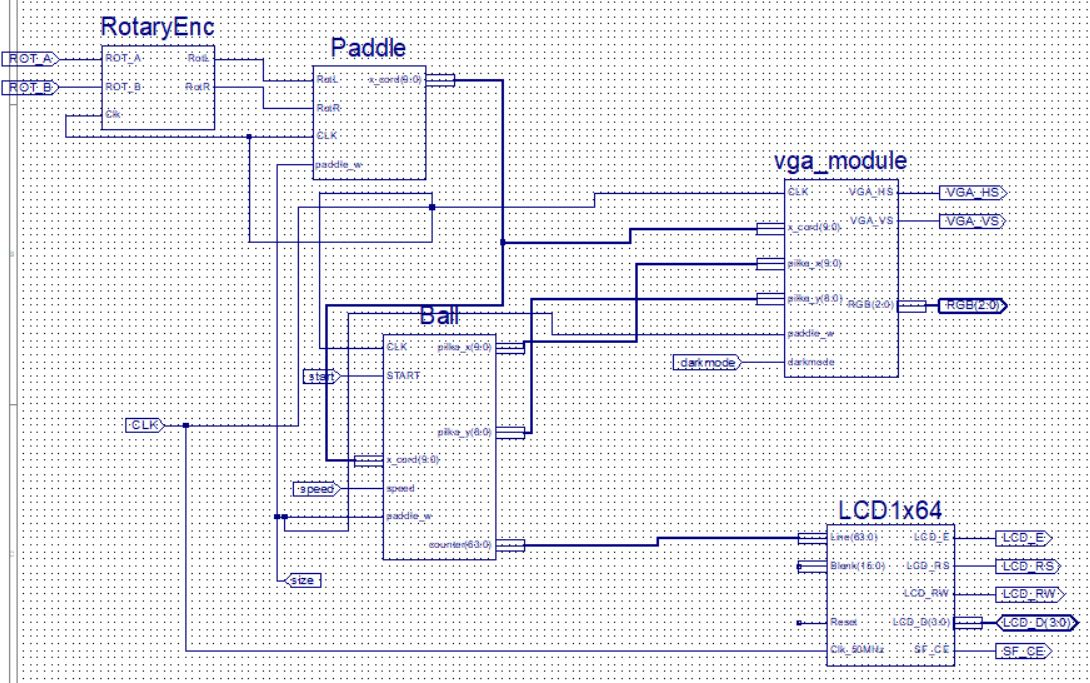
\includegraphics[height=8cm]{schemat2.JPG}  
    \caption{Główny schemat}
    \label{fig:my_label}
\end{figure}

\subsection{Moduł Ball}
\subsubsection{Opis}
Moduł Ball odpowiada za mechanikę piłki, to znaczy:
\begin{itemize}
    \item poruszanie się piłki po ekranie;
    \item sprawdzanie odbicia z paletką;
    \item sprawdzanie przegranej.
    \item zatrzymanie piłki
\end{itemize}

\subsubsection{Schemat}


\lstinputlisting[caption={Sygnały modułu Ball},captionpos=b,firstline=32, lastline=42]{ball.vhd}

\begin{figure}[h!]
    \centering
    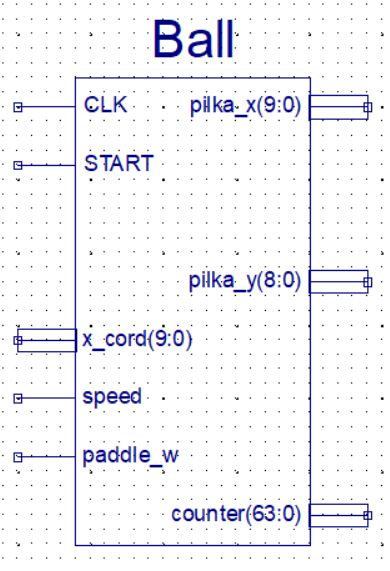
\includegraphics[height=8cm]{ball.JPG}  
    \caption{Schemat modułu Ball}
    \label{fig:my_label}
\end{figure}



\begin{itemize}
    \item CLK - zegar 50 MHz
    \item START - start/zatrzymanie ruchu piłki
    \item x\_cord - współrzędna paletki
    \item speed - wybór szybkości piłki
    \item paddle\_w - szerokość paletki
    \item pilka\_x - współrzędna x piłki
    \item pilka\_y - współrzędna y piłki
    \item counter - licznik odbić
\end{itemize}

\newpage
\subsubsection{Kod}
\lstset{style=vhdl}
\lstinputlisting[caption={Sprawdzenie odbicia z paletką}, captionpos=b, firstline=111, lastline=134]{ball.vhd}
\newpage
  
\subsection{Moduł Paddle}
\subsubsection{Opis}
Moduł Paddle obsługuje mechanikę paletki, to znaczy:

\begin{itemize}
    \item zmianę położenia paletki przy pomocy Rotary Encoder;
    \item przekazywanie współrzędnych paletki do modułu wyświetlającego.
\end{itemize}

\subsubsection{Schemat}

\lstinputlisting[caption={Sygnały modułu Paddle},captionpos=b,firstline=32, lastline=38]{paddle.vhd}

\begin{figure}[ht]
    \centering
    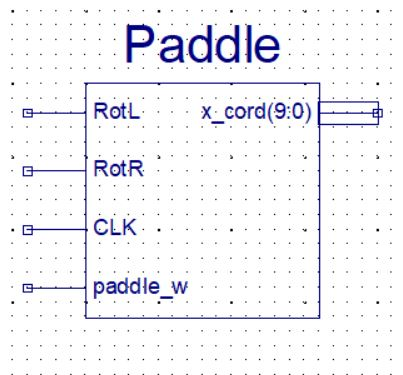
\includegraphics[height=8cm]{paddle.JPG}  
    \caption{Schemat modułu Paddle}
    \label{fig:my_label}
\end{figure}


  
\begin{itemize}
    \item RotL - sygnał ruchu w lewo
    \item RotR - sygnał ruchu w prawo
    \item CLK - zegar 50 MHz
    \item paddle\_w - szerokość paletki
     \item x\_cord - współrzędna paletki
\end{itemize}

\subsubsection{Kod}
\lstset{style=vhdl}
\lstinputlisting[caption={Zmiana położenia paletki},captionpos=b,firstline=56, lastline=81]{paddle.vhd}
  
\newpage
\subsection{Moduł VGA\_Module}
\subsubsection{Opis}
Moduł VGA\_Module obsługuje wyświetlanie na monitorze VGA oraz zmianę kolorów wyświetlania.

Moduł VGA\_Module generuje sygnały czasowe oraz synchronizacyjne. Sygnały h\_sync oraz v\_sync są służą do kontrolowania poziomych oraz pionowych skanów monitora. Te dwa sygnały są dekodowane przez wewnętrzny licznik, którego wyjściem są sygnały
h\_counter x oraz v\_counter. Sygnały wyjściowe wskazują na względną pozycję skanowania i określają położenie bieżącego piksela.

\subsubsection{Schemat}

\lstset{style=vhdl}
\lstinputlisting[caption={Sygnały modułu VGA\_Module},captionpos=b,firstline=32, lastline=42]{vgamodule.vhd}

\begin{figure}[ht]
    \centering
    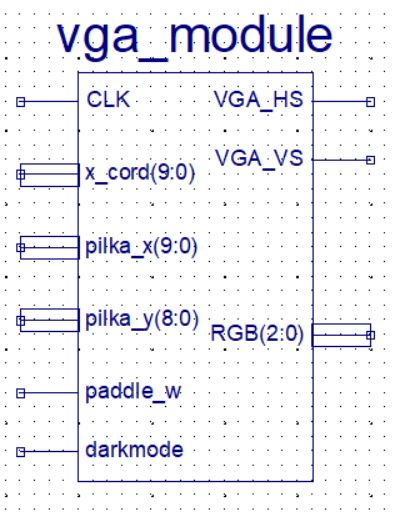
\includegraphics[height=8cm]{vga_module.JPG}  
    \caption{Schemat modułu VGA\_Module}
    \label{fig:my_label}
\end{figure}
\begin{itemize}
    \item CLK - zegar 50 MHz
    \item x\_cord - współrzędna paletki
    \item pilka\_x - współrzędna x piłki
    \item pilka\_y - współrzędna y piłki
    \item paddle\_w - szerokość paletki
    \item darkmode - wybór ciemnego motywu
    \item VGA\_HS - sygnał synchronizacji poziomej
    \item VGA\_VS - sygnał synchronizacji pionowej
    \item RGB - kolor piksela
\end{itemize}

\subsubsection{Kod}
\lstset{style=vhdl}
\lstinputlisting[caption={Synchronizacja pozioma},captionpos=b,firstline=116, lastline=127]{vgamodule.vhd}
\newpage

\lstset{style=vhdl}
\lstinputlisting[caption={Licznik położenia w poziomie},captionpos=b,firstline=94, lastline=112]{vgamodule.vhd}

\lstset{style=vhdl}
\lstinputlisting[caption={Rysowanie obiektów na ekranie},captionpos=b,firstline=163, lastline=191]{vgamodule.vhd}

\subsection{Inne moduły}
Dodatkowo w projekcie znalazły się gotowe moduły obsługujące enkoder rotacyjny (RotaryEnc), za pomocą którego poruszana jest paletka oraz wyświetlacz LCD (LCD1x64), za pomocą którego wyświetlana jest liczba odbić piłki. Oba moduły pochodzą ze strony internetowej \newline$www.zsk.ict.pwr.wroc.pl/zsk\_ftp/fpga/$. 

\section{Wnioski}
Logika gry została przeniesiona do modułu Ball (początkowo miała znajdować się w module VGA\_Module). Nie udało się wykonać zliczania punktów, jedynie zliczanie odbić w postaci hexadecymalnej na wyświetlaczu LCD. Podczas wykonywania projektu zmagaliśmy się z problemem z wyświetlaniem, który zajął nam 2 zajęcia projektowe. Problem był skomplikowany do wykrycia, ponieważ był on związany z konwersją STD\_LOGIC\_VECTOR na signed\_integer. Podczas konwersji należy pamiętać, że zmienia się zakres liczby i zamiast np. liczby od 0 do 255 uzyskujemy liczbę od -127 do 128. Problem został ostatecznie rozwiązany ale zabrał dużo czasu.
\end{document}